\ifacita
\else
% I'm convinced by Peter's examples of min / max total mass being
% useful.  It will be interesting to see what types of calculations end
% up being most prevalent in our examples.  The interplay between total
% mass and the per-point mass function is interesting and seems like the
% sort of thing that mathematicians may have considered before.  I did
% some minor digging and Simplexes seem related:

% http://en.wikipedia.org/wiki/Simplex
% (also see http://en.wikipedia.org/wiki/Categorical_distribution)

% As a bonus, n-dimensional simplexes correspond directly to
% n-dimensional convex polyhedra.  One big difference between our
% distribution sets and simplexes is that we have bounds on the number
% of 0-valued points.

% Anyway, something to think about after we get this paper written.  I
% suspect there is a large space of possible abstractions for these
% distributions and it will be interesting to compare them (once we
% discover them :-)

\section{Belief revision via abstract interpretation}
\label{sec:absinterp}

\setlength{\arraycolsep}{0.1cm}
\newcommand{\ajoin}[0]{\bigsqcup}

% We could implement the belief semantics described in the previous
% section more-or-less directly, e.g., using an existing probabilistic
% language (such as IBAL~\cite{pfeffer07ibal} or Probabilistic
% Scheme~\cite{radul07probscheme}).  However, existing approaches use
% sampling to perform belief revisions, and for the examples of the sort
% given in Section~\ref{sec:examples}, the input space is too large for
% sampling to compute sound answers efficiently.  Therefore, we have
% developed a probabilistic semantics using abstract
% interpretation.

Consider how we might implement belief tracking and revision to enforce the
threshold security property given in Definition~\ref{def:threshold}.  A
natural choice would be to evaluate queries using a probabilistic
programming language with support for conditioning; examples are
IBAL~\cite{pfeffer07ibal}, Probabilistic
Scheme~\cite{radul07probscheme}, and several
others~\cite{park08sampling,goodman08church,kiselyov09embedded}.  In  
these languages, probabilistic evaluation is achieved by enumerating
inputs (sampling).  Probabilities are associated with each input and tracked during
execution.  As more inputs are enumerated, a more complete view of
the output distribution emerges.  Unfortunately,
to get an accurate estimate of the revised distribution following an output observation,
one must enumerate the
entire input space, which could be quite large.  If insufficient coverage is
achieved, then the threshold check in Definition~\ref{def:threshold} could
either be unsound or excessively conservative, depending in which direction
an implementation errs.

To avoid sampling, we have developed a new means to perform probabilistic
computation based on abstract interpretation.  In this approach, execution time
depends on the complexity of the query rather than the size of the input space.
In the next two sections, we
present two abstract domains.  This section presents the first, denoted
$\ppolys$, where an abstract element is a single \emph{probabilistic
  polyhedron}, which is a convex polyhedron~\cite{CousotHalbwachs78-POPL}
with information about the probabilities of its points.  Because using
a single polyhedron will accumulate imprecision after multiple queries, in our
implementation we actually use a different domain, denoted $ \ppowers $, for
which an abstract element consists of a set of at most $n$ probabilistic
polyhedra (whose construction is inspired by powersets of polyhedra
\cite{bagnara06powerset,Popeea06inferringdisjunctive}).  This domain, described in the next section,
allows us to retain precision at the cost of increased execution time.  By
adjusting $n$, the user can trade off efficiency and precision.

\subsection{Polyhedra}

We first review \emph{convex polyhedra}, a common technique for representing sets of program states.  We use the meta-variables $\ineq, \ineq_1, \ineq_2$, etc. to denote linear inequalities.  We write $\fv\ineq$ to be the set of variables occurring in
$\ineq$; we also extend this to sets, writing $\fv{\{\ineq_1,\ldots,\ineq_n\}}$ for $\fv{\ineq_1} \cup \ldots \cup \fv{\ineq_n}$.

\begin{definition}
  A \emph{convex polyhedron} $\poly = (\cons, V)$ is a set of linear inequalities
  $\cons = \{\ineq_1,\ldots,\ineq_m\}$, interpreted conjunctively,
  over dimensions $ V $.  We write
  $\cp$ for the set of all convex polyhedra.   A polyhedron $\poly$
  represents a set of states, denoted $\pconc{\poly}$, as follows, where $\sigma \models \ineq$ indicates that the state $\sigma$ satisfies the inequality $\ineq$.
\[\pconc{\paren{\cons,V}} \defeq \{\sigma \mid \dom\sigma =
V \;,\; \forall \ineq \in \cons.\ \sigma \models \ineq\}\]

Naturally we require that $\fv{\{\ineq_1,\ldots,\ineq_n\}} \subseteq V
$. We write $ \fv{\paren{\cons, V}} $ to denote the set of variables $
V $ of a polyhedron.

\end{definition}

% Figure \ref{fig:polyhedra} gives an example of a
% polyhedron $\poly$ and the set of states $\pconc{\poly}$.
Given a state $\sigma$ and an ordering on the variables in $\dom{\sigma}$, we can view $\sigma$ as a point in
an $N$-dimensional space, where $N = \setsize{\dom\sigma}$.  The set $\pconc{\poly}$ can then be viewed as the integer-valued lattice points in an $N$-dimensional polyhedron.
Due to this correspondence, we use the words \textit{point} and
\textit{state} interchangeably.  We will sometimes write linear equalities $x = f(\vec{y})$ as an abbreviation for the pair of inequalities $x \leq f(\vec{y})$ and $x \geq f(\vec{y})$.
% \todo{TODO: draw this picture.}

\newcommand{\myitem}{~\\ \noindent $\bullet$ }
Let $ \poly = (\cons, V) $. Convex polyhedra support the following
operations.
% \begin{itemize}
%   We
% write $\setsize{S}$ to represent the cardinality of the set $S$.
\myitem{} Polyhedron size, or $ \psize{\poly} $, is the number of
   integer points in the polyhedron, i.e., $\setsize{\pconc{\poly}}$.
   We will always consider bounded polyhedra when determining their
   size, ensuring that $\psize{\poly}$ is finite.
\myitem{} Expression evaluation, $\abseeval{\bexp}{\poly}$ returns a
   convex polyhedron containing at least the points in $\poly$ that satisfy
$\bexp$.
\myitem{} Expression count, $\absecount{\bexp}{\poly}$ returns an upper bound
 on the number of integer points in $\poly$ that satisfy $\bexp$.  (It
 may be more precise than $\psize{\abseeval{\bexp}{\poly}}$.)
% \sbmcomment{Because these are abstract operations (and may be approximate).
% $\absecount{\bexp}{\poly} \leq \psize{\abseeval{\bexp}{\poly}}$ but they may
% not be equal (and will not be for polyhedra).  Image the condition $\neg(x = 0)$.
% If $\poly$ is $-5 \leq x \leq 5$ then $\abseeval{\bexp}{\poly}$ is $-5 \leq x \leq 5$,
% which has 11 points, while $\absecount{\bexp}{\poly}$ could return $10$.
% Our implementation of $\absecount{\bexp}{\poly}$ proceeds by introducing some
% disjunction (thus retaining more precision) before doing the counting.  So it would count
% the points in the two polyhedra given by $-5 \leq x \leq -1$ and $1 \leq x \leq 5$.
% (These disjuncts can then either be thrown away or kept, depending on whether we are
% in the single polyhedron domain or the powerset domain.)
% While we implement a rather roundabout way of computing points consistent with $\bexp$
% (introduce disjunctions, take intersections, count),
% it's possible that a more direct method could be devised.  In any case, given the fact
% that considering this operation separately can improve precision, it seemed worth keeping
% it separate.  It also corresponds nicely with $\abseeval{\bexp}{\poly}$ (which is
% more precise than its ``naive'' implementation as $\poly \pmeet \alpha(\bexp)$, where
% $\alpha$ is the abstraction function returning the smallest convex polyhedron containing $\bexp$).
% }
 \myitem{} Meet, $ \pa \pmeet \pb $ is the convex
 polyhedron containing exactly the set of points in the intersection of
 $\pconc{\pa}, \pconc{\pb}$.
\myitem{} Join, $\pa \pjoin \pb$ is the smallest convex
 polyhedron containing both $\gamma(\pa)$ and $\gamma(\pb)$.
\myitem{} Comparison, $\pa \pord \pb$ is a partial order whereby $\pa \pord \pb$ if and only if $\gamma(\pa) \subseteq \gamma(\pb)$.
\myitem{} Affine transform, $\poly \bparen{x \ra \aexp}$, where $x
  \in \fv{\poly} $, computes an affine transformation of $ \poly $.  This scales
  the dimension corresponding to $x$ by the coefficient of $x$ in
  $\aexp$ and shifts the polyhedron.  For example, $\paren{\{x \leq y, y =
  2z\}, V} \bparen{y \ra z + y}$ evaluates to $\paren{\{x \leq y - z, y - z =
  2z\}, V}$.
\myitem{} Forget, $\forget{x}{\poly}$, projects
  away $x$.  That is, $\forget{x}{\poly} =
  \pi_{\fv{\poly}-\{x\}}(\poly)$, where $\pi_V(\poly)$ is a polyhedron
  $\poly'$ such that $\pconc{\poly'} = \{ \sigma \mid \sigma' \in
  \pconc{\poly} \wedge \sigma = \project{\sigma'}{V} \}$.  So $\poly' =
  \forget{x}{\poly}$ implies $x \not\in fv(\poly')$.
%\item{} Add dimensions, $ \newdim{V'}{\poly} $ is the polyhedron with
%  additional dimensions $ V' $ that are disjoint from $ \fv{\poly} $. Thus $
%  \fv{\newdim{V'}{\poly}} = \fv{\poly} \cup V' $ with the dimensions $ V'
%  $ unconstrained. If $ V' = \set{x_1, \cdots, x_m} $ then $
%  \pconc{\newdim{V'}{C}} = \set{\sigma \cup \set{x_i = n_i}_{i=1}^{m}
%    \given \sigma \in \pconc{C}, n_i \in \Integer} $.  We write $
%  \sigma \cup \set{x = n} $ to denote a state $ \sigma $ with an
%  additional assignment of $ x $ to value $ n $. \pxm{check this}
% \end{itemize}

We write $\isempty{\poly}$ \emph{iff} $\pconc{\poly} = \emptyset$.

% We write $\emptypoly$ to denote the empty polyhedron.  We have
% $\pconc{\emptypoly} = \emptyset$ and any polyhedron with an
% inconsistent set of linear constraints is equivalent to
% $\emptypoly$. \mwh{What is $\fv{\emptypoly}$?  Perhaps it's $\vars$,
%   or any $V \subseteq \vars$?}

\subsection{Probabilistic Polyhedra}

We take this standard representation of sets of program states and
extend it to a representation for sets of distributions over program
states.  We define \emph{probabilistic polyhedra}, the core element of
our abstract domain, as follows.

\begin{definition}
A \emph{probabilistic polyhedron} $\pp{}$ is a tuple
$(\getpoly{},\smin{}, \smax{}, \pmin{}, \pmax{}, \mmin{}, \mmax{})$.  
We write $\ppolys$ for the set of probabilistic polyhedra.  The
quantities $\smin{}$ and $ \smax{}$ are lower and upper bounds on 
the number of support points in the polyhedron $\getpoly{}$.  The quantities
$\pmin{} $ and $ \pmax{} $ are lower and upper bounds on the
probability mass \emph{per support point}.  The $ \mmin{} $ and $
\mmax{} $ components give bounds on the total probability mass.  
Thus $\pp{}$ represents the \emph{set} of distributions
$\ppconc{\pp{}}$ defined below. 
\[
\ppconc{\pp{}} \defeq
\begin{aligned}[t]
\{\delta \mid {} & \nzset{\delta} \subseteq \pconc{\getpoly{}} \wedge {} \\
  & \smin{} \leq \setsize{\nzset{\delta}} \leq \smax{} \wedge {} \\
  & \mmin{} \leq \pmass{\delta} \leq \mmax{} \wedge \\
  & \forall \sigma \in \nzset{\delta}.\ \pmin{} \leq \delta(\sigma) \leq \pmax{}\}
\end{aligned}
\]

We will write $ \fv{\pp{}} \defeq \fv{\poly} $ to denote the set of variables
used in the probabilistic polyhedron. 

\end{definition}
% Recall that $\pmass{\delta}$ gives the mass of distribution $\delta$,
% which is the sum of the probabilities ascribed to states by $\delta$. 
Note the set $\ppconc{\pp{}}$ is singleton exactly when $\smin{} = \smax{}
= \psize{\getpoly{}}$ and $\pmin{} = \pmax{}$, and $\mmin{} =
\mmax{}$.  In such a case $\ppconc{\pp{}}$ is the uniform distribution
where each state in $\pconc{\getpoly{}}$ has probability $\pmin{}$.
Distributions represented by a probabilistic polyhedron are not
necessarily normalized (as was true in
Section~\ref{sec:clarkson-semantics}).  In general, there is a
relationship between $\pmin{}, \smin{}, $ and $\mmin{}$, in that
$\mmin{} \geq \pmin{} \cdot \smin{}$ (and $\mmax{} \leq \pmax{} \cdot
\smax{}$), and the combination of the three can yield more information
than any two in isolation.

Our convention will be to use $\getpoly{1}$, $\smin{1}$, $\smax{1}$,
etc. for the components associated with probabilistic polyhedron
$\pp{1}$ and to use subscripts to name different probabilistic
polyhedra.

% Figure
% \ref{fig:pp-ex} gives an example of the 
% relationship between distributions and probabilistic polyhedra.
% Note that the set $\ppconc{\pp{}}$ is singleton exactly when
% $\smin{} = \smax{} = \psize{\getpoly{}}$ and $\pmin{} = \pmax{}$, and $\mmin{} = \mmax{}$.
% In such a case $\ppconc{\pp{}}$ is the uniform distribution where each state
% in $\pconc{\getpoly{}}$ has probability $\pmin{}$.  Consistent with the discussion of
% distributions in Section \ref{sec:clarkson-semantics}, the distributions represented
% by a probabilistic polyhedron are not necessarily
% normalized. \mwh{make sure we're clear in \ref{sec:distributions}
%   about this.}

Distributions are ordered point-wise~\cite{clarkson09quantifying}.
That is, $\delta_1 \leq \delta_2$ if and only if $\forall
\sigma.\ \delta_1(\sigma) \leq \delta_2(\sigma)$.  For
our abstract domain, we say that $\pp{1} \ppord \pp{2}$ if and only if
$\forall \delta_1 \in \ppconc{\pp{1}}.\ \exists \delta_2 \in
\ppconc{\pp{2}}.\ \delta_1 \leq \delta_2$.  Testing $\pp{1} \ppord
\pp{2}$ mechanically is non-trivial, but is unnecessary in our
semantics.  Rather, we need to test whether a distribution
represents only the zero distribution $\distzero \defeq \lambda
\sigma. 0$ in order to see that a fixed point for evaluating
$\abspevalp{\swhile{\bexp}{\stmt}}{\pp{}}$ has been reached.
Intuitively, no further iterations of the loop need to be considered
once the probability mass flowing into the $n^\text{th}$ iteration is
zero. This condition can be detected as follows:

\vspace*{-0.9em}
\begin{small}
\[
\begin{array}{l}
\iszero{\pp{}} \defeq \\
\qquad \smin{} = \smax{} = 0 \wedge \mmin{} = 0 \leq \mmax{} \\
\quad \vee\; \mmin{} = \mmax{} = 0 \wedge \smin{} = 0 \leq \smax{} \\
\quad \vee\; \isempty{\poly} \wedge \smin{} = 0 \leq \smax{} \wedge
\mmin{} = 0 \leq \mmax{} \\
\quad \vee\; \pmin{} = \pmax{} = 0 \wedge \smin{} = 0 \leq \smax{} \wedge
\mmin{} = 0 \leq \mmax{} \\
\end{array}
\]
\end{small}
If $ \iszero{\pp{}} $ holds, it is the case that $ \ppconc{\pp{}} =
\set{\distzero} $. Note that having a more conservative
definition of this function (which holds for fewer probabilistic polyhedra)
would be reasonable since it would simply
mean our analysis would terminate less often than it could, with no
effect on security.  \iffull More details are given in Appendix~\ref{appendix:proof1}.
\else More details are given in our technical report~\cite{TR}. \fi

In a standard abstract domain, termination of the
fixed point computation for loops is often ensured by use of a widening
operator.  This allows abstract fixed points to be computed in fewer
iterations and also permits analysis of loops that may not terminate.
In our setting, non-termination may reveal information about secret
values.  As such, we would like to reject queries that may be non-terminating.

We enforce this by not introducing a widening operator.  Our abstract
interpretation then has the property that it will not terminate if a loop
in the query may be non-terminating
(and, since it is an over-approximate analysis, it may also fail to terminate
even for some terminating computations).  We then reject all queries for
which our analysis fails to terminate.
Loops do not play a major role
in any of our examples, and so this approach has proved sufficient so far.
We leave for future work the development of a widening operator that soundly
accounts for non-termination behavior.

Following standard abstract interpretation terminology, we will refer to $\powerset{\dists}$ (sets of distributions) as the \textit{concrete domain}, $\ppolys$ as the \textit{abstract domain}, and $\ppconcfun : \ppolys \rightarrow \powerset{\dists}$ as the \textit{concretization function} for $\ppolys$.

\subsection{Abstract Semantics for $\ppolys$}

To support execution in the abstract domain just defined, we need
to provide abstract implementations of the basic operations of assignment,
conditioning, addition, and scaling used in the concrete semantics given in
Figure \ref{fig-sem-nondet2-core}.  We will overload notation and use the
same syntax for the abstract operators as we did for the concrete operators.

As we present each operation, we will also state the associated
soundness theorem which shows that the abstract operation is an
over-approximation of the concrete operation.  
\iffull
Proofs are given in Appendix~\ref{appendix:proof1}.
\else
Proofs are given in our technical report~\cite{TR}.
\fi
The abstract program
semantics is then exactly the semantics from Figure
\ref{fig-sem-nondet2-core}, but making use of the abstract operations
defined here, rather than the operations on distributions defined in Section \ref{sec:clarkson-semantics}.
We will write
$\abspevalp{S}{\pp{}}$ to denote the result of executing $S$ using the
abstract semantics.  The main soundness theorem we obtain is the following.
\begin{theorem}
\label{thm:pp:soundness}
For all $\pp{}, \delta$, if $ \delta \in \ppconc{\pp{}} $ and
$ \abspevalp{S}{\pp{}} $ terminates, then $ \pevalp{S}{\delta} $ terminates and $
\pevalp{S}{\delta} \in \ppconc{\abspevalp{S}{\pp{}}} $.
\end{theorem}

When we say $ \pevalp{S}{\delta} $ terminates (or  $ \abspevalp{S}{\pp{}} $
terminates) we mean that only a finite number of loop unrollings are
required to interpret the statement on a particular distribution (or
probabilistic polyhedron).
\iffull
The precise
definitions of termination can be found in Appendix~\ref{appendix:proof1}. 
\else
The precise definitions of termination are given in the technical
report~\cite{TR}.
\fi

We now present the abstract operations.

\subsubsection{Forget}

We first describe the abstract forget operator $\forget{y}{\pp{1}}$, which is used in
implementing assignment.  When we forget variable $y$, we collapse any
states that are equivalent up to the value of $y$ into a single state.
To do this correctly, we must find an upper bound $\maxh{y}$ and a lower bound $\minh{y}$
on the number of points that share the same value of other dimensions $x$ (this may be visualized of as the min and max height of $\getpoly{1}$ in the $y$ dimension).
Once these are obtained, we have that $\forget{y}{\pp{1}} \defeq \pp{2}$ where the following hold of $\pp{2}$.
\[
\begin{array}{lcl@{\hspace{0.4cm}}|@{\hspace{0.4cm}}lcl}
\poly_2 &=& \multicolumn{4}{l}{\forget{y}{\poly_1}} \bigstrut[b] \\
\pmin{2} &=& \multicolumn{4}{l}{\pmin{1} \cdot \maxparen{\minh{y}-(\psize{\poly_1} - \smin{1}),\ 1}} \bigstrut \\
\pmax{2} &=& \multicolumn{4}{l}{\pmax{1} \cdot \minparen{\maxh{y},\ \smax{1}}} \bigstrut \\
\smin{2} &=& \lceil{\smin{1} / \maxh{y}}\rceil &
  \mmin{2} &=& \mmin{1} \bigstrut \\
\smax{2} &=& \minparen{\psize{\forget{y}{\poly_1}},\ \smax{1}} &
  \mmax{2} &=& \mmax{1} \bigstrut[t]
\end{array}
\]

\begin{figure}
\begin{center}
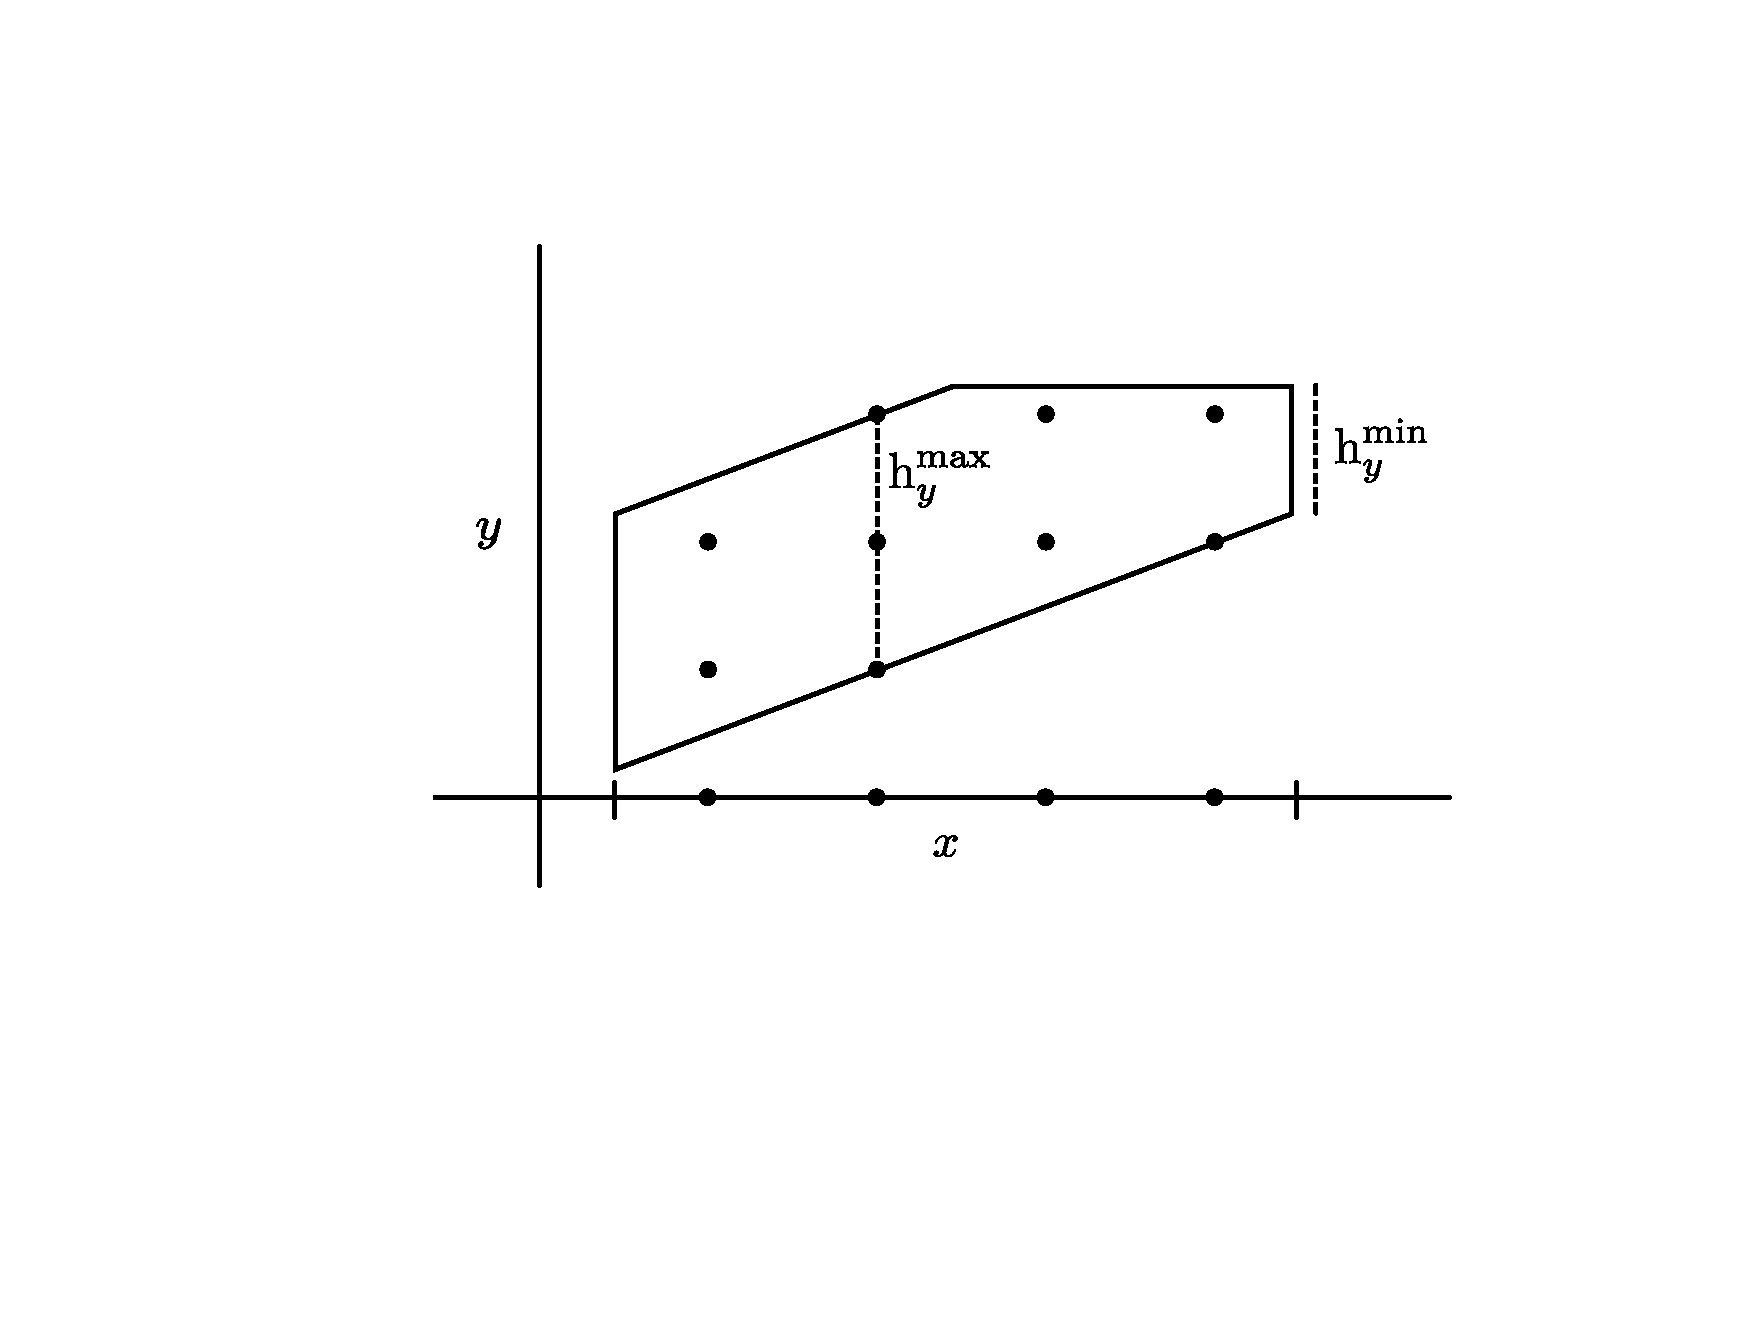
\includegraphics[width=6.5cm]{figures/forget.pdf} % !!! commented out slow figure
\end{center}
\caption{\label{fig:forget} Example of a forget operation in the abstract domain $\ppolys$.  In this case, $\minh{y} = 1$ and $\maxh{y} = 3$.  Note that $\maxh{y}$ is precise while $\minh{y}$ is an under-approximation.  If $\smin{1} = \smax{1} = 9$ then we have $\smin{2} = 3$, $\smax{2} = 4$, $\pmin{2} = \pmin{1} \cdot 1$, $\pmax{2} = \pmax{2} \cdot 4$.}
\end{figure}

Figure \ref{fig:forget} gives an example of a forget operation and
illustrates the quantities $\maxh{y}$ and $\minh{y}$.  If $ \poly_1 =
(\cons_1, V_1) $, the upper bound $\maxh{y}$ can be found by maximizing $y - y'$ subject to the
constraints $\cons_1 \cup \cons_1[y' / y]$, where $y'$ is a fresh variable and $\cons_1[y'/y]$ represents the set of
constraints obtained by substituting $y'$ for $y$ in $\cons_1$.  As our
points are integer-valued, this is an integer linear programming
problem (and can be solved by ILP solvers).  A less precise upper bound
can be found by simply taking the extent of the polyhedron $\getpoly{1}$ along $y$,
which is given by $\psize{\pi_y(\getpoly{1})}$.

For the lower bound, it is always sound to use $\minh{y} = 1$, which is what our implementation does.  A more precise estimate can be obtained by finding the vertex with minimal height along dimension $y$.  Call this distance $u$.  Since the shape is convex, all other points will have $y$ height greater than or equal to $u$.  We then find the smallest number of integer points that can be covered by a line segment of length $u$.  This is given by $\lceil u \rceil - 1$.  This value can be taken as $\minh{y}$.

Since the forget operator is related to projection, we state soundness
in terms of the projection operation on distributions.  Note that
$\fv{\delta} \defeq \dom{\dom{\delta}}$, i.e., the domain of 
states to which $\delta$ assigns probability mass.
\begin{lemma}
\label{lem:pp:forget}
If $\delta \in \ppconc{\pp{}}$ then $\project{\delta}{(\fv{\delta} - \{y\})} \in \ppconc{\forget{y}{\pp{}}}$.
\end{lemma}
\noindent
We can define an abstract version of projection using forget:
\begin{definition}
Let $\forget{\{x_1,x_2,\ldots,x_n\}}{\pp{}} =
\forget{\{x_2,\ldots,x_n\}}{\forget{x_1}{\pp{}}}$.  Then
$\project{\pp{}}{V'} = \forget{(\dom{\pp{}} - V')}{\pp{}}$. 
\end{definition}
That is, in order to project onto the set of variables $V'$, we forget all variables not in $V'$.

\subsubsection{Assignment}

We have two cases for abstract assignment.  If 
\iffull
$\sassign{x}{E}$ is invertible,\footnote{See Appendix~\ref{appendix:proof1} for a
  precise definition of invertibility.}
\else
$\sassign{x}{E}$ is invertible,
\fi
% \footnote{An assignment
%   $\sassign{x}{E}$ is invertible if 
%   and only if there is some $E'$ such that for all $\sigma$, if
% $\sigma' = \sigma \bparen{x \ra \evalp{E}\sigma}$ then 
% $\sigma' \bparen{x \ra \evalp{E'}{\sigma'}} = \sigma$. \mwh{Drop
%   this, and copy from the appendix}} 
the
 result of the assignment $\pp{1} \bparen{x \ra E}$ is the
probabilistic polyhedron $\pp{2}$ such that
$\getpoly{2} = \getpoly{1} \bparen{x \ra E}$ and all other
components are unchanged.

If the assignment is not invertible, then information about
the previous value of $x$ is lost.  In this case, we use the forget
operation to project onto the other variables and then add a new
constraint on $x$.  Let $\pp{2} = \forget{x}{\pp{1}}$
where $\poly_2 = (\cons_2, V_2)$.  Then $\pp{1}
\bparen{x \ra E}$ is the probabilistic polyhedron $\pp{3}$ with 
$ \poly_3 = (\cons_2 \cup \set{x = E}, V_2 \cup \set{x})$ and all
other components as in $\pp{2}$.

\begin{lemma}
\label{lem:pp:assign}
If $\delta \in \ppconc{\pp{}}$ then $\delta \bparen{v \ra \aexp} \in \ppconc{\pp{} \bparen{v \ra \aexp}}$.
\end{lemma}

The soundness of assignment relies on the fact that our
language of expressions does not include division.  An invariant of
our representation is that $\smax{} \leq \psize{\poly}$.  
% That is,
% there can never be more than $\psize{\poly}$ support points in a
% probabilistic polyhedron with polyhedral portion $\poly$.  
When $E$ contains only multiplication and addition the
above rules preserve this invariant; an $E$ containing division would
violate it. 
Division would collapse multiple points to one and so could be handled
similarly to projection.

\subsubsection{Plus}

% We illustrate abstract plus with the example in Figure
% \ref{fig:pplus}, which shows two overlapping probabilistic polyhedra.  
To soundly compute the effect of plus we need to determine the minimum
and maximum number 
of points in the intersection that may be a support point for both
$\ppa$ and for $\ppb$.  We refer to these counts as the
\emph{pessimistic overlap} and \emph{optimistic overlap},
respectively, and define them below.

\begin{definition}
\label{def:abs-overlap}
  Given two distributions $\delta_1,\delta_2$, we refer to the set of
  states that are in the support of both $\delta_1$ and $\delta_2$ as
  the \emph{overlap} of $\delta_1,\delta_2$.  The \emph{pessimistic
    overlap} of $\ppa$ and $\ppb$, denoted $\pessoverlap{\ppa}{\ppb}$,
  is the cardinality of the smallest possible overlap for any distributions
  $\delta_1 \in \ppconc{\ppa}$ and $\delta_2 \in \ppconc{\ppb}$.  The
  \emph{optimistic overlap} $\optoverlap{\ppa}{\ppb}$ is the cardinality of the largest possible
  overlap.  Formally, we define these as follows.  $n_3 \defeq \psize{\pa
    \pmeet \pb} \bigstrut[b]$, $n_1 \defeq \psize{\pa} - n_3 \bigstrut$, and
  $n_2 \defeq \psize{\pb} - n_3 \bigstrut[t]$.  Then
\[\begin{array}{l}
\pessoverlap{\ppa}{\ppb} \defeq \maxparen{(\smin{1} - n_1) + (\smin{2} - n_2) -
n_3,\ 0} \\
\optoverlap{\ppa}{\ppb} \defeq \minparen{\smax{1}, \smax{2}, n_3} \\
\end{array}\]
\end{definition}
We can now define abstract addition.

\begin{definition}
\label{def:pplus}
If not $ \iszero{\pp{1}} $ and not $ \iszero{\pp{2}} $ then $\ppa \ppplus \ppb$ is the probabilistic polyhedron $\pp{3} = (\getpoly{3},\smin{3},\smax{3},\pmin{3},\pmax{3})$ defined as follows.
\[
\begin{array}{lcl}
\getpoly{3} &=& \pa \pjoin \pb \bigstrut \\
\pmin{3} &=& 
\begin{cases}
\pmin{1} + \pmin{2} & \text{if } \pessoverlap{\ppa}{\ppb} = \psize{\getpoly{3}} \bigstrut[t] \\
\minparen{\pmin{1}, \pmin{2}} & \text{otherwise}\bigstrut[b] 
\end{cases} \bigstrut \\

\pmax{3} &=&
\begin{cases}
\pmax{1} + \pmax{2} & \text{if } \optoverlap{\ppa}{\ppb} > 0 \bigstrut[t] \\
\maxparen{\pmax{1}, \pmax{2}} & \text{otherwise}\bigstrut[b]
\end{cases} \bigstrut \\

\smin{3} &=& \maxparen{\smin{1} + \smin{2} - \optoverlap{\ppa}{\ppb},
  \; 0} \bigstrut \\

\smax{3} &=& \minparen{\smax{1} + \smax{2} - \pessoverlap{\ppa}{\ppb},
\; \psize{\getpoly{3}}} \bigstrut \\

\mmin{3} &=& \mmin{1} + \mmin{2} \bigstrut \quad \mid \quad
\mmax{3} = \mmax{1} + \mmax{2} \bigstrut  \\
\end{array}
\]
% \pxm{added a check to smin above to make sure it cannot get below
%   zero}
% \pxm{added a check to smax being no bigger than content of polyhedron,
%   TODO: make the appropriate note in the proof in the appendix}

If $ \iszero{\pp{1}}$ then we define $ \ppa \ppplus \ppb $ as identical 
to $ \ppb $; if $ \iszero{\pp{2}} $, the sum is defined as
identical to $ \pp{1} $. 
\end{definition}

\begin{lemma}
\label{lem:pp:plus}
If $\delta_1 \in \ppconc{\pp{1}}$ and $\delta_2 \in \ppconc{\pp{2}}$ then $\delta_1 + \delta_2 \in \ppconc{\pp{1} + \pp{2}}$.
\end{lemma}

\deleted{
\subsubsection{Abstract Union (aka Join)}
 
We next define our abstract join operation, which approximates the set operation $D_1 \cup D_2$.
 
\begin{definition}
The \emph{abstract join} of probabilistic polyhedra $\ppa$ and $\ppb$,
denoted $\ppa \ppcup \ppb$, is the probabilistic polyhedron $\ppc =
(P_3,\pmin{3},\pmax{3},\smin{3},\smax{3})$ defined as follows.
\begin{itemize}
\item{} $ \poly_3 = \pa \pjoin \pb $
\item{} $ \pmin{3} = \minparen{\pmin{1},\pmin{2}}$
\item{} $ \pmax{3} = \maxparen{\pmax{1},\pmax{2}}$
\item{} $ \smin{3} = \minparen{\smin{1},\smin{2}}$
\item{} $ \smax{3} = \maxparen{\smax{1},\smax{2}}$
\end{itemize}
\end{definition}
}

\subsubsection{Product}
When evaluating the product $\pp{3} = \pp{1} \times \pp{2}$, we assume
that the domains of $\pp{1}$ and $\pp{2}$ are disjoint, i.e.,
$\poly_1$ and $\poly_2$ refer to disjoint sets of 
variables.  If $ \poly_1 = (\cons_1, V_1) $ and $ \poly_2 = (\cons_2,
V_2) $, then the polyhedron $\poly_1 \pprod \poly_2 \defeq
\paren{\cons_1 \cup \cons_2, V_1 \cup V_2}$ is the Cartesian product
of $\poly_1$ and $\poly_2$ and contains all those states $\sigma$ for
which $\project{\sigma}{V_1} \in \pconc{\poly_1}$ and
$\project{\sigma}{V_2} \in \pconc{\poly_2}$. 
% \pxm{changed the poly
%   product notation to not be confused with union of constraints and
%   gave the exact definition} 
Determining the remaining components is straightforward since $\pp{1}$
and $\pp{2}$ are disjoint. 
\[
\begin{array}{rcl@{\hspace{0.35cm}}|@{\hspace{0.35cm}}rcl}
\multicolumn{6}{c}{\poly_3\ =\ \poly_1 \pprod \poly_2} \bigstrut[b] \\
\pmin{3} &=& \pmin{1} \cdot \pmin{2} &
\pmax{3} &=& \pmax{1} \cdot \pmax{2} \bigstrut \\
\smin{3} &=& \smin{1} \cdot \smin{2} &
\smax{3} &=& \smax{1} \cdot \smax{2} \bigstrut \\
\mmin{3} &=& \mmin{1} \cdot \mmin{2} &
\mmax{3} &=& \mmax{1} \cdot \mmax{2} \bigstrut[t]
\end{array}
\]

\begin{lemma}
\label{lem:pp:product}
For all $\pp{1}, \pp{2}$ such that $\fv{\pp{1}} \cap
\fv{\pp{2}} = \emptyset$, if $\delta_1 \in \ppconc{\pp{1}}$ and
$\delta_2 \in \ppconc{\pp{2}}$ then $\delta_1 \times \delta_2
\in \ppconc{\pp{1} \times \pp{2}}$. 
\end{lemma}

In our examples we often find it useful to express uniformly distributed
data directly, rather than encoding it using $\spifk$.  In particular,
consider extending statements $S$ to include the statement form
$\suniform{x}{n_1}{n_2}$ whose semantics is to define variable $x$ as
having values uniformly distributed between $n_1$ and $n_2$.
Its semantics is as follows.
$$
\begin{array}{rcl}
\abspevalp{\suniform{x}{n_1}{n_2}}{\pp{1}} & = & \forget{x}{\pp{1}}
\times \pp{2}
\end{array}
$$
Here, $ \pp{2} $ has $ \pmin{2} = \pmax{2} = \frac{1}{n_2 - n_1 + 1}
$, $ \smin{2} = \smax{2} = n_2 - n_1 + 1 $, $ \mmin{2} = \mmax{2} = 1
$, and $ C_2 = (\set{x \geq n_1, x \leq n_2}, \set{x}) $.

We will say that the abstract semantics correspond to the concrete
semantics of $ \suniformname $ defined similarly as follows.
$$
\begin{array}{rcl}
\pevalp{\suniform{x}{n_1}{n_2}}{\delta} & = &
\paren{\project{\delta}{\fv{\delta} - \set{x}}} \times \delta_2
\end{array}
$$
where $ \delta_2 = (\lambda \sigma. \aif n_1 \leq \sigma(x)
\leq n_2 \athen \frac{1}{n_2 - n_1 + 1} \aelse 0)$.

The soundness of the abstract semantics follows immediately from the
soundness of forget and product.

\subsubsection{Conditioning}

\newcommand{\nn}{\overline{n}} 
\newcommand{\nnu}{\underline{n}} 

Distribution conditioning for probabilistic polyhedra serves the same
role as meet in the classic domain of polyhedra in that each is used
to perform abstract evaluation of a conditional expression in its
respective domain.

\begin{definition}
  Consider the probabilistic polyhedron $\ppa$ and Boolean expression
  $\bexp$.  Let $n,\nn$ be such that $n = \absecount{\bexp}{\getpoly{1}}$ and
  $\nn = \absecount{(\neg\bexp)}{\getpoly{1}}$.  
The value $n$ is an over-approximation of the number of points in
$\getpoly{1}$ that satisfy the condition $\bexp$ and $\nn$ is an
over-approximation of the number of points in $\getpoly{1}$ that do
not satisfy $\bexp$.
Then $\absdcond{\ppa}{\bexp}$ is the probabilistic polyhedron $\ppb$
  defined as follows.

\vspace*{-0.9em}
\begin{small}
\[
\setlength{\arraycolsep}{1pt}
\begin{array}{lcl@{\hspace{0.35cm}}|@{\hspace{0.35cm}}lcl}
\pmin{2} &=& \pmin{1} &
\smin{2}\ &=&\ \maxparen{\smin{1} - \nn, 0}\\
\pmax{2} &=& \pmax{1} \bigstrut[b] &
\smax{2} &=&\ \minparen{\smax{1}, n} \bigstrut \\
%\mmin{2} &=& \multicolumn{4}{l}{\max\tparen{\pmin{2} \cdot
%\smin{2},\ \mmin{1} - \pmax{1} \cdot \nn}} \bigstrut\\
\mmin{2} &=& \multicolumn{4}{l}{\maxparen{\pmin{2} \cdot
    \smin{2},\ \mmin{1} - \pmax{1} \cdot \minparen{\smax{1}, \nn}}} \bigstrut\\
%\mmax{2} &=& \multicolumn{4}{l}{\min\tparen{\pmax{2} \cdot
%\smax{2},\ \mmax{1} - \pmin{1} \cdot \nnu}} \bigstrut\\
\mmax{2} &=& \multicolumn{4}{l}{\minparen{\pmax{2} \cdot
    \smax{2},\ \mmax{1} - \pmin{1} \cdot \maxparen{\smin{1}-n, 0}}} \bigstrut\\
\getpoly{2} &=& \multicolumn{4}{l}{\abseeval{\bexp}{\pa}} \bigstrut[t] \\
\end{array}
\]
\end{small}
\end{definition}
% It is easy to see that if $\iszero{\pp{1}}$ then $\iszero{\pp{2}}$.
% \mwh{Note comment about $\iszero{\pp{1}}$ case}

The maximal and minimal probability per point
are unchanged, as conditioning simply retains points from
the original distribution.  To compute the minimal number of points in
$\pp{2}$, we assume that
as many points as possible from $\getpoly{1}$ fall in the region
satisfying $\neg\bexp$.  The maximal number of points is obtained by
assuming that a maximal number of points fall within the region
satisfying $\bexp$.

The total mass calculations are more complicated.  
There are two
possible approaches to computing $\mmin{2}$ and $\mmax{2}$.  The bound
$\mmin{2}$ can never be less than $\pmin{2} \cdot \smin{2}$, and so we
can always safely choose this as the value of $\mmin{2}$.  Similarly,
we can always choose $\pmax{2} \cdot \smax{2}$ as the value of
$\mmax{2}$.  However, if $\mmin{1}$ and $\mmax{1}$ give good bounds on
total mass (i.e., $\mmin{1}$ is much higher than $\pmin{1} \cdot
\smin{1}$ and dually for $\mmax{1}$), then it can be advantageous
to reason starting from these bounds.

We can obtain a sound value for $\mmin{2}$ by considering
the case where a maximal amount of mass from $\getpoly{1}$
fails to satisfy $B$.  To do this, we compute
$\nn = \absecount{\neg\bexp}{\getpoly{1}}$, which provides an
over-approximation of the number of points within $\getpoly{1}$ but
outside the area satisfying $B$.  We bound $\nn$ by $\smax{1}$ and then assign each of
these points maximal mass $\pmax{1}$, and subtract this
from $\mmin{1}$, the previous lower bound on total mass.

By similar reasoning, we can compute $\mmax{2}$ by assuming a minimal amount
of mass $m$ is removed by conditioning, and subtracting $m$
from $\mmax{1}$.  This $m$ is given by
considering an under-approximation of the number of points falling
outside the area of overlap between $\getpoly{1}$ and $B$ and assigning
each point minimal mass as
given by $\pmin{1}$.  This $m$ is given by $\max\tparen{\smin{1}-n, 0}$.

\begin{figure}
\begin{center}
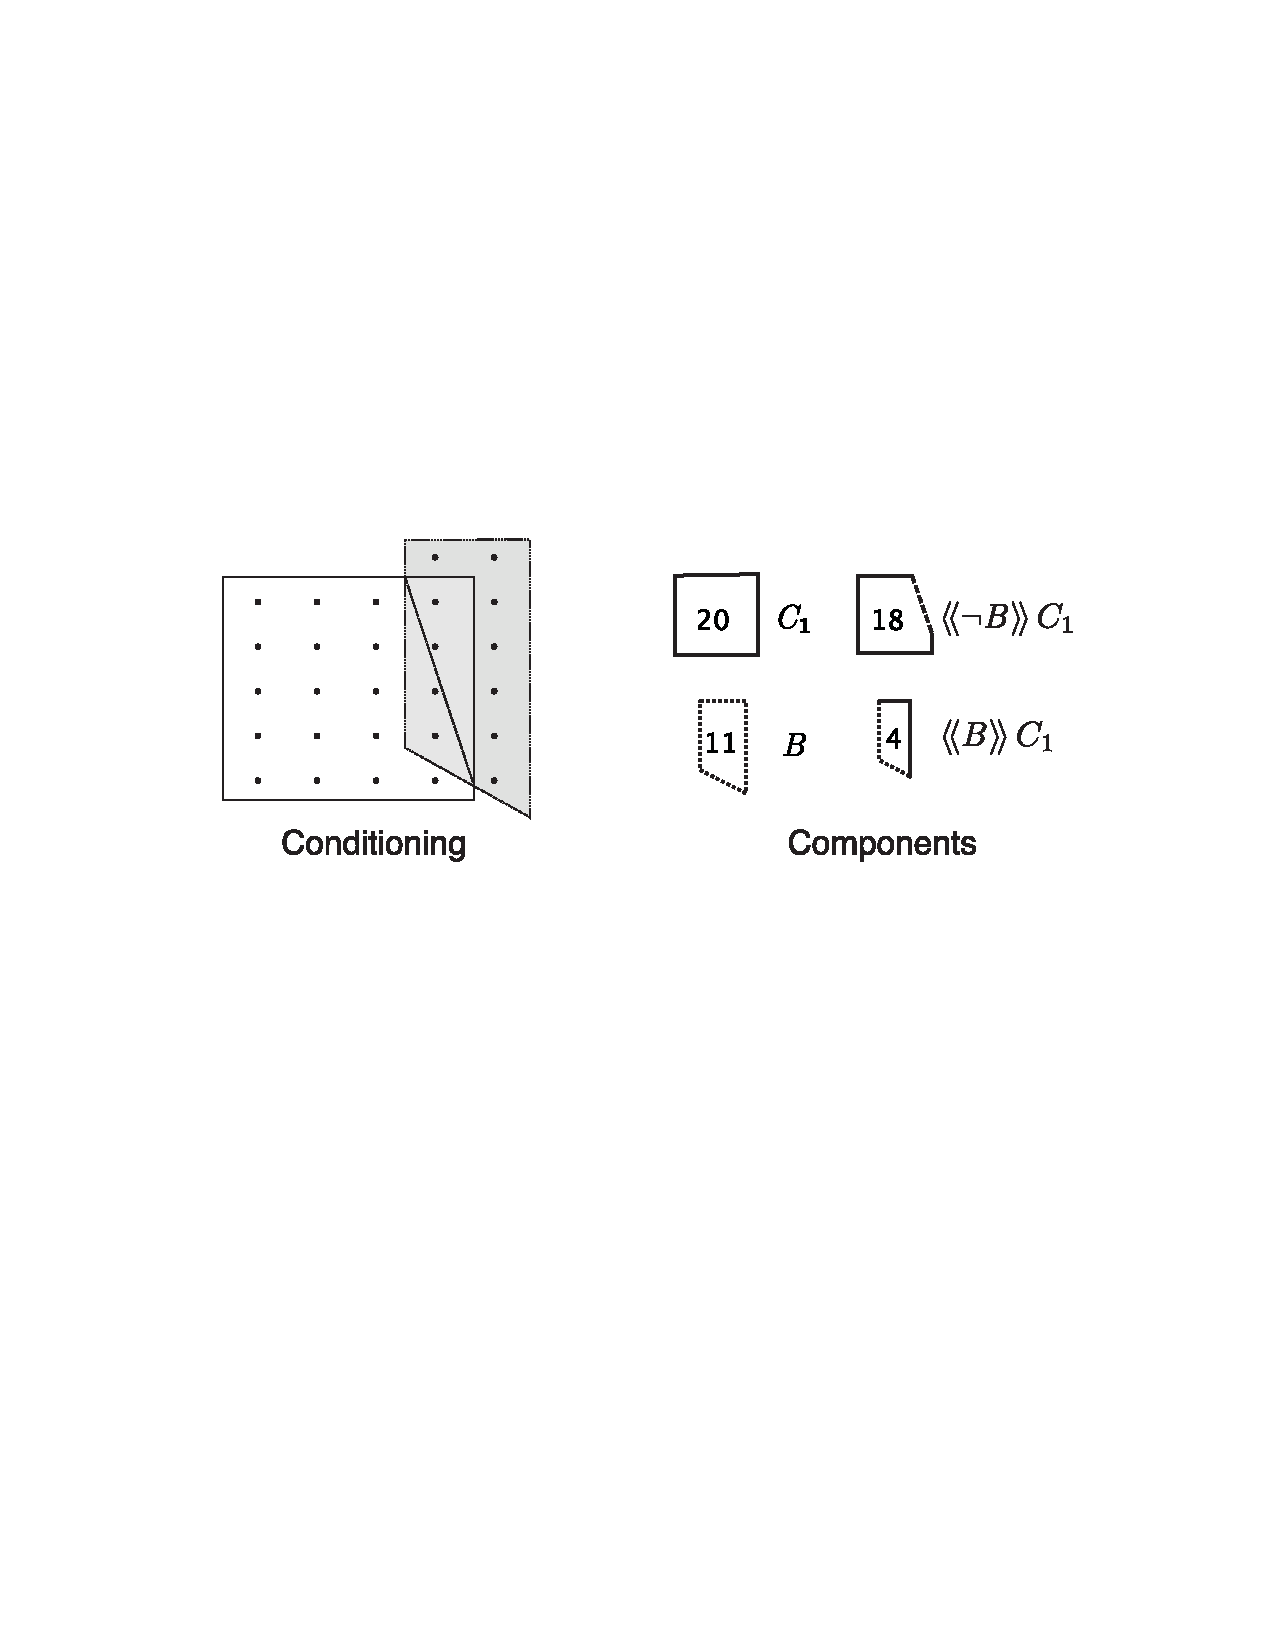
\includegraphics[width=7.5cm]{figures/conditioning-smaller.pdf}
\end{center}
\caption{\label{fig:conditioning} Example of distribution conditioning in the abstract domain $\ppolys$.}
\end{figure}

Figure \ref{fig:conditioning} demonstrates the components that affect the
conditioning operation.  The figure depicts the integer-valued points
present in two polyhedra---one representing $\getpoly{1}$ and the other
representing $\bexp$ (shaded).  As the set of points in $\getpoly{1}$
satisfying $\bexp$ is convex, 
this region is precisely represented by $\abseeval{\bexp}{\getpoly{1}}$.  By contrast, the set of points
in $\getpoly{1}$ that satisfy $\neg\bexp$ is not convex, and thus $\abseeval{\neg\bexp}{\getpoly{1}}$ is an
over-approximation.  The icons
beside the main image indicate which shapes correspond to which components
and the numbers within the icons give the total count of points within those
shapes.

Suppose the components of $\pp{1}$ are as follows.
\[
\begin{array}{l@{\qquad}l@{\qquad}l}
\smin{1} = 19 & \pmin{1} = 0.01 & \mmin{1} = 0.85 \\
\smax{1} = 20 & \pmax{1} = 0.05 & \mmax{1} = 0.9
\end{array}
\]
Then $n = 4$ and $\nn = 16$.  Note that we have set $\nn$ to be the
number of points in the non-shaded region of Figure \ref{fig:conditioning}.
This is more precise than the count given by $\psize{\abseeval{\bexp}{\poly}}$, which
would yield $18$.  This demonstrates why it is worthwhile to have a
separate operation for counting points satisfying a boolean expression.
These values of $n$ and $\nn$ give us the following for
the first four numeric components of $\pp{2}$.
\[
\begin{array}{l@{\qquad}l}
\smin{2} = \max(19 - 16, 0) = 3 & \pmin{2} = 0.01 \\
\smax{2} = \min(20,4) = 4 & \pmax{2} = 0.05
\end{array}
\]
For the $\mmin{2}$ and $\mmax{2}$, we have the following for the
method of calculation based on $\mathrm{p^{min/max}_2}$ and
$\mathrm{s^{min/max}_2}$.
\[
\begin{array}{l@{\qquad}l}
\mmin{2} = 0.01 \cdot 3 = 0.03  & \mmax{2} = 0.05 \cdot 4 = 0.2
\end{array}
\]
For the method of computation based on $\mathrm{m^{min/max}_1}$, we have
\[
\begin{array}{llcrr}
\mmin{2} &= &0.85 - 0.05 \cdot 16& =& 0.05\\
 \mmax{2} &= &0.9 - 0.01 \cdot (19-4)& =& 0.75
\end{array}
\]

In this case, the calculation based on subtracting from total mass
provides a tighter estimate for $\mmin{2}$, while the method based on
multiplying $\pmax{2}$ and $\smax{2}$ is better for
$\mmax{2}$.

\begin{lemma} \label{lem:pp:cond} If $ \delta \in \ppconc{\pp{}} $ then $
  \dcond{\delta}{B} \in \ppconc{\absdcond{\pp{}}{B}} $.
\end{lemma}


% \paragraph{Benefits of dual mass representations}

% The total minimum mass of a probabilistic polyhedron can seemingly be
% determined using two redundant means: either $ \mmin{} $ or $ \pmin{}\cdot \smin{} $. Tracking the measure in these two ways, however, is useful for
% keeping the measure accurate. For some abstract operations one of
% these means is more accurate than the other.

% Any abstract plus operation involving probabilistic polyhedra having
% two different minimum probability per point measures, the total mass
% based approach is more accurate, or equivalently accurate in the rare
% case where the minimum number of points is identical to the number of
% points in the polyhedra.

% \sbmcomment{It might be easier to read if we convert the fractions to decimals.}

% \begin{example} Consider two disjoint probabilistic polyhedra $ \ppa $, $ \ppb $,
% with the following characteristics:

% $ \pmin{1} = \frac{1}{100} $

% $ \smin{1} = 10 $

% $ \mmin{1} = \frac{10}{100} $

% $ \pmin{2} = \frac{1}{200} $

% $ \smin{2} = 20 $

% $ \mmin{2} = \frac{20}{100} $

% $ \pa \cap \pb = \emptyset $

% The abstract plus of the two, $ \ppc := \ppa \ppplus \ppb $ has the
% following properties.

% $ \pmin{3} = \frac{1}{200} $

% $ \smin{3} = 30  $

% $ \mmin{3} = \frac{30}{100} $

% Note that $ \pmin{3} \cdot \smin{3} = \frac{15}{100} $, a more inaccurate
% measure than $ \mmin{3} = \frac{30}{100} $.
% \end{example}

% The difference in the two total mass approaches stems from the need to
% under-approximate both minimum probability per point from both
% polyhedra with a single value.

% For abstract plus, the total mass approach always produces more
% accurate results but in the case of abstract revision, the approach
% can, in some cases, produce results worse than the $ \pmin{}\cdot \smin{} $ approach. First let us look at an example in which the total mass is
% still more accurate.

% \begin{example} Consider a probabilistic polyhedron $ \ppa $ and a
% polyhedron $ \pb $ where the intersection between the two is quite
% large in relation to the size of $ \pa $. 

% $ \pmin{1} = \frac{1}{1000} $

% $ \pmax{1} = \frac{1}{100} $

% $ \smin{1} = 95 $

% $ \mmin{1} = \frac{20}{100} $

% Furthermore, $ \setsize{\pa} - \setsize{\pa \cap \pb} = 10 $ and
% $ \setsize{\pa \cap \pb} = 90 $. That is, the $ \pa $ contains 100
% points, 90 of which are in the intersection with $ \pb $.

% To determine the total mass of $ \ppc := \absdcond{\ppa}{\pb} $ we
% reason that a maximum amount of mass falls outside the intersection,
% corresponding to $ \pmax{1} \cdot \paren{\setsize{\pa}
% - \setsize{\pa \cap \pb}} = \frac{1}{100} \cdot 10 $ .  \sbmcomment{I think you mean \textit{minimal} total mass here.}
% Thus the total
% mass of the intersection would be $ \mmin{1} - \frac{10}{100}
% = \frac{10}{100} $. On the other hand, $ \pmin{3} \cdot \smin{3}
% = \frac{1}{1000} \cdot 85 < \frac{10}{100} $.
% \end{example}

% As seen in the example above, the calculation of total mass derives
% it's accuracy from the maximum estimates as applied to the area
% outside of the intersection. If, however, this area is instead large,
% we see that this approach fails.

% \begin{example}

% Consider a probabilistic polyhedron $ \ppa $ and a
% polyhedron $ \pb $ where the intersection between the two is small in relation to the size of $ \pa $. 

% $ \pmin{1} = \frac{1}{1000} $

% $ \pmax{1} = \frac{1}{100} $

% $ \smin{1} = 95 $

% $ \mmin{1} = \frac{20}{100} $

% Furthermore, $ \setsize{\pa} - \setsize{\pa \cap \pb} = 90 $ and
% $ \setsize{\pa \cap \pb} = 10 $. That is, the $ \pa $ contains 100
% points, 10 of which are in the intersection with $ \pb $.

% To determine the total mass of $ \ppc := \absdcond{\ppa}{\pb} $ we
% reason that a maximum amount of mass falls outside the intersection,
% corresponding to $ \pmax{1} \cdot \paren{\setsize{\pa}
% - \setsize{\pa \cap \pb}} = \frac{1}{100} \cdot 90 $ . Thus the total
% mass of the intersection would be $ \mmin{1} - \frac{90}{100}
% = - \frac{70}{200} $, or simply a value having no use whatsoever. On the other hand, $ \pmin{3} \cdot \smin{3}
% = \frac{85}{1000} $. In such a case, we let $ \mmin{3}
% := \pmin{3} \cdot \smin{3} $ in order for the total mass measure to have
% potential usefulness in further computation.
% \end{example} 

% \pxm{todo: perhaps it would be nice to provide programs that actually
% give rise to the examples above}

\subsubsection{Scalar Product}
The scalar product is straightforward, as it just scales the mass per point and total mass.

\begin{definition}
Given a scalar $p$ in $[0,1]$, we write $p \cdot \ppa$ for the probabilistic polyhedron $\ppb$ specified below.
\[
\begin{array}{lcl@{\hspace{0.5cm}}|@{\hspace{0.5cm}}lcl}
\smin{2} &=& \smin{1} & \pmin{2} &=& p \cdot \pmin{1} \\
\smax{2} &=& \smax{1} & \pmax{2} &=& p \cdot \pmax{1} \\
\mmin{2} &=& p \cdot \mmin{1} & \getpoly{2} &=& \getpoly{1}\\
\mmax{2} &=& p \cdot \mmax{1} 
\end{array}
\]
% Observe that when $ p = 0 $, then $\iszero{\pp{2}}$ (assuming that
% $\pp{1}$ is consistent). \mwh{Had to add this parenthetical assumption of
%   consistency to make the statement true; just make it this by
%   definition instead?}
% \pxm{changes here, needed special case for the minimum
%   number of points to be sound}
% \sbmcomment{Changed this to just be $\ppzero$, rather than list all the components.}
% \sbmcomment{But also, note that the definition assumes $p$ cannot be
%   $0$.  Given that, can we eliminate the special case, or do we want
%   to allow $p$ to be $0$?} \mwh{Probably should change the definition,
%   for completeness}
\end{definition}

\begin{lemma}
\label{lem:pp:scalar-prod}
If $\delta_1 \in \ppconc{\pp{1}}$ then $p \cdot \delta_1 \in \ppconc{p \cdot \pp{1}}$.
\end{lemma}

\subsubsection{Normalization}

If a probabilistic polyhedron $\pp{}$ has $\mmin{} = 1$ and $\mmax{} =
1$ then it represents a normalized distribution.  We define below an
abstract counterpart to distribution normalization, capable of
transforming an arbitrary probabilistic polyhedron into one containing
only normalized distributions.
% , with the property that if $\delta \in
% \ppconc{\pp{}}$ then $\normal{\delta} \in \ppconc{\normal{\pp{}}}$.
% This ensures that $\normal{\pp{}}$ is a sound over-approximation of
% $\normal{\delta}$ for the purposes of policy evaluation.

\begin{definition}
Whenever $ \mmin{1} > 0 $, we write $\normal{\pp{1}}$ for the probabilistic polyhedron $\pp{2}$
specified below.
\[
\begin{array}{lcl@{\hspace{0.35cm}}|@{\hspace{0.35cm}}lcl}
\pmin{2} &=& \pmin{1} / \mmax{1} &
\smin{2} &=& \smin{1}\\
\pmax{2} &=& \pmax{1} / \mmin{1} &
\smax{2} &=&\smax{1} \\
\mmin{2} &=& \mmax{2} = 1 & \getpoly{2} &=& \getpoly{1} \\
\end{array}
\]
\end{definition}

When $ \mmin{1} = 0 $, we set $\pmax{2} = 1$.  Note that if $\pp{1}$
is the zero distribution then $\normal{\pp{1}}$ is not defined.

%\pxm{todo: resolve this issue: $ \mmin{2} = \frac{\mmin{1}}{\mmin{1}} $ or $ \mmin{2} = \frac{\mmin{1}}{\mmax{1}} $}

\begin{lemma}
\label{lem:pp:norm}
If $\delta_1 \in \ppconc{\pp{1}}$ and $\normal{\delta_1}$ is defined, then $\normal{\delta_1} \in \ppconc{\normal{\pp{1}}}$.
\end{lemma}

\subsection{Policy Evaluation}

\noindent Here we show how to implement the threshold test given as
Definition \ref{def:threshold} using probabilistic polyhedra. To make
the definition simpler, let us first introduce a bit of notation.

\begin{notation} If $ \pp{} $ is a probabilistic polyhedron over
  variables $ V $, and $
  \sigma $ is a state over variables $ V' \subseteq V $, then $ \absdcond{\pp{}}{\sigma} \defeq
  \absdcond{\pp{}}{\bexp} $ where $ \bexp = \bigwedge_{x \in V'} x =
  \sigma(x) $.
\end{notation}

\begin{definition}
Given some probabilistic polyhedron $\pp{1}$ and statement $S$ where
$\abspevalp{S}{\pp{1}} $ terminates, let
$\pp{2} = \abspevalp{S}{\pp{1}}$ and $\pp{3} =
\project{\pp{2}}{L}$. If, for every $ \sigma_L \in \pconc{\getpoly{3}}
$ with $ \neg\iszero{\absdcond{\pp{2}}{\sigma_L}}$, we have
$ \pp{4} =
\normal{\project{\paren{\absdcond{\pp{2}}{\sigma_L}}}{H}} $ 
with $\pmax{4} \leq t$, then we
write $\abspolicy{S}{\pp{1}}{t}$.
\end{definition}

The computation of $\pp{3}$ involves only abstract interpretation and
projection, which are computable using the operations defined previously
in this section.  If we have a small number of outputs (as for the binary outputs
considered in our examples), we can enumerate them and check
$\neg\iszero{\absdcond{\pp{2}}{\sigma_L}}$ for each output $\sigma_L$.
When this holds (that is, the output is feasible), we compute $\pp{4}$,
which again simply involves the abstract operations defined previously.
The final threshold check is then performed by comparing $\pmax{4}$ to
the probability threshold $t$.

% Notice the number of revisions required depends on the size
% of $\pconc{\getpoly{3}}$; in our earlier examples the size is two, with
% $\sigma = \{ (\var{output},\sconst{True}) \}$ or $\sigma = \{
% (\var{output}, \sconst{False}) \}$.  \mwh{Say more? Less?}

Now we state the main soundness theorem for abstract interpretation
using probabilistic polyhedra.  This theorem states that the abstract
interpretation just described can be used to soundly determine whether
to accept a query.

\begin{theorem} \label{thm:pp:secure}
  Let $\delta$ be an attacker's initial belief.  If $\delta \in
  \ppconc{\pp{1}}$ and $\abspolicy{S}{\pp{1}}{t}$, then $S$ is threshold secure
  for threshold $t$ when evaluated with initial belief $\delta$.
\end{theorem}

\deleted{
\sbmcomment{TODO: fix up this proof}
\begin{proof}
We have from Theorem \ref{thm:pp:soundness} that if $\delta_1 \in \ppconc{\pp{1}}$ and $(\pevalp{S}{\delta_1}) = \delta_2$ and $\pp{2} = \abspevalp{S}{\pp{1}}$ then $\delta_2 \in \ppconc{\pp{2}}$.  Combined with Lemma \ref{lem:pp:norm} this gives us that $\normal{\delta_2} \in \ppconc{\normal{\pp{2}}}$.  Let $\delta_3 = \normal{\delta_2}$ and $\pp{3} = \normal{\pp{2}}$.  Since every element $\delta'$ of $\ppconc{\pp{3}}$ satisfies $\delta'(\sigma) \leq \pmax{3}$ for all $\sigma$, and $\delta_3 \in \pconc{\pp{3}}$, we have that $\delta_3(\sigma) \leq \pmax{3}$ for all $\sigma$.  Since we also have $\pmax{3} \leq t$, this implies that $\forall \sigma.\ \delta_3(\sigma) \leq t$ and thus $S$ is threshold secure.
\end{proof}
}

\deleted{
The following is not a soundness theorem, but rather shows that an
invariant of our representation is preserved.

\begin{theorem}
If $\mmin{1} \geq \pmin{1} \cdot \smin{1}$ and $\mmin{2} \geq \pmin{2} \cdot \smin{2}$ and $\pp{3} = \pp{1} + \pp{2}$ then $\mmin{3} \geq \pmin{3} \cdot \smin{3}$.
\end{theorem}
\sbmcomment{
Also holds for $\mmax{3}, \pmax{3}, \smax{3}$ and for other abstract
operations.  This answers the question of whether we ever need to
``fix up'' our representation by using $\pmin{}, \smin{}$ to find a
tighter bound on $\mmin{}$.}

\sbmcomment{
One question that is still open:  Do we ever need to ``fix up'' $\pmin{}$ by reasoning that
\[\mmin{} - \pmax{} \cdot (\smax{} - 1) \leq \pmin{}\]
or equivalently
\[\mmin{} \leq \pmin{} + \pmax{} \cdot (\smax{} - 1)\]
}

\sbmcomment{Revised through here.  Next we need to talk about normalization and how probabilistic polyhedra relate to the various entropy measures we are interested in.}

\mwh{Want to prove that semantics maintains a sound over-approximation of the
  probabilities of the concrete distribution, so that threshold policies are
  preserved.}

\sbmcomment{TODO: Revise powerset below to be consistent with discussion of singleton abstraction above.}
\sbmcomment{TODO: Talk about projection and merging---the two ways that precision can be lost when working in the powerset domain.}
\sbmcomment{TODO: Talk about precision loss when merging elements of the powerset and give the formula we use to approximate precision loss.}
}

\section{Powerset of Probabilistic Polyhedra}
\label{sec:probset}

This section presents the $ \ppowers $ domain, an extension of the $ \ppolys
$ domain 
that abstractly represents a set of distributions as at most $ n $
probabilistic polyhedra, elements of $ \ppolys $.

\begin{definition} A \emph{probabilistic (polyhedral) set} $
  \pps{} $ is a set of probabilistic polyhedra, or  $ \set{\pp{i}} $
  with each $ \pp{i} $ over the same variables. We write $
  \ppowers $ for the domain of probabilistic polyhedral powersets
  composed of no more than $ n $ probabilistic polyhedra.

Each probabilistic polyhedron $\pp{}$ is interpreted disjunctively: it
characterizes one of many possible distributions.  The probabilistic
polyhedral set is interpreted additively.  To define this idea
precisely, we first define a lifting of $+$ to sets of distributions.  Let $\distset{1}, \distset{2}$ be two sets of distributions.  We then define addition as follows.
\[\distset{1} + \distset{2} = \{\delta_1 + \delta_2 \mid \delta_1 \in \distset{1} \wedge \delta_2 \in \distset{2}\}\]
This operation is commutative and associative and thus we can use $\sum$ for summations without ambiguity as to order of operations.
The concretization function for $\ppowers$ is then defined as:
$$ \ppsconc{\pps{}} \defeq \sum_{\pp{} \in \pps{}} \ppconc{\pp{}} $$
\end{definition}

We can characterize the condition of $ \pps{} $ containing only the
zero distribution, written $ \iszero{\pps{}} $, via the condition that
all of the member probabilistic polyhedra are zero.
$$ \iszero{\pps{}} \defeq \bigwedge_{\pp{} \in \pps{}} \iszero{\pp{}} $$

\deleted{
\begin{definition} $ \delta_a = \delta_b $ if and only if $ \forall \sigma $ $
  \delta_a(\sigma) = \delta_b(\sigma) $.
\end{definition}
}

\subsection{Abstract Semantics for $\ppowers$}

With a few exceptions, the abstract implementations of the basic
operations for the powerset domain are extensions of operations
defined on the base probabilistic polyhedra domain.

\begin{theorem} \label{thm:ppp:soundness}
For all $\delta, S, \pps{}$, if $\delta \in \ppsconc{\pps{}}$ and $
\abspevalp{S}{\pps{}} $ terminates, then $ \pevalp{S}{\delta} $ terminates and
$\pevalp{S}{\delta} \in
\ppsconc{\abspevalp{S}{\pps{}}}$.
\end{theorem}

\iffull
Proof of this theorem is given in Appendix~\ref{appendix:proof2}.
\fi

\begin{definition}
\label{def:ppp-simp}
The \emph{powerset simplification} transforms a
  set containing potentially more than $ n $ elements into one
  containing no more than $ n $, for $n \geq 1$. The simplest approach involves repeated use
  of abstract plus in the base domain $ \ppolys $.
$$
\simplify{\set{\pp{i}}_{i=1}^{m}}{n} \defeq \left\{
\begin{array}{cc}
\set{\pp{i}}_{i=1}^{m} & \text{if } m \leq n \\
\simplify{\set{\pp{i}}_{i=1}^{m-2} \cup \set{\pp{m-1} + \pp{m}}}{n} & \text{otherwise} \\
\end{array}
\right.
$$
\end{definition}

\begin{lemma}
\label{lem:ppp:bound}
$ \ppsconc{\pps{}} \subseteq \ppsconc{
    \simplify{\pps{}}{m}} $ where $m \leq n$.
\end{lemma}

Note that the order in which individual probabilistic
polyhedra are simplified has no effect on soundness but may impact the
precision of the resulting abstraction.

Many of the operations and lemmas for the powerset domain are simple liftings
of the corresponding operations and lemmas for single probabilistic polyhedra.
For these operations (operations 1-5 given below), we simply list the
definition.

\subsubsection{Forget} $ \forget{y}{\pps{}} \defeq
\set{\forget{y}{\pp{}} \mid \pp{} \in \pps{}} $

\subsubsection{Project} $ \project{\pps{}}{V} \defeq
\set{\project{\pp{}}{V} \mid \pp{} \in \pps{}} $

\subsubsection{Conditioning} $ \absdcond{\pps{}}{B} \defeq
\set{\absdcond{\pp{}}{B} \mid \pp{} \in \pps{}} $

% \begin{lemma} 
% If $ \delta \in \ppsconc{\pps{}} $ then $
%   \project{\delta}{\paren{\fv{\delta} - \set{y}}} \in
%   \ppsconc{\forget{y}{\pps{}}} $
% \end{lemma}

\subsubsection{Assignment} $ \pps{} \bparen{x \ra E} \defeq
  \set{\pp{} \bparen{x \ra E} \mid \pp{} \in \pps{}} $

% \begin{lemma} If $ \delta \in \ppsconc{\pps{}} $ then $
%   \delta\bparen{x \ra E} \in \ppsconc{\pps{} \bparen{x \ra E}} $.
% \end{lemma}

\subsubsection{Scalar product} $ p \cdot \pps{} \defeq \set{p
  \cdot \pp{} \mid \pp{} \in \pps{}} $

% \begin{lemma} If $ \delta \in \ppsconc{\pps{}} $ then $
%   p \cdot \delta \in \ppsconc{p \cdot \pps{}} $.
% \end{lemma}

\subsubsection{Product} The product operation is only required for the
special $ \suniformname $ statement and only applies to the product
of a probabilistic set with a single probabilistic polyhedron.
$ \pps{} \times \pp{}' \defeq \set{\pp{} \times \pp{}' \mid \pp{} \in \pps{}} $
(where we assume that $\fv{\pps{}} \cap \pp{}' = \emptyset$).

% \pxm{does this need a lemma?}

% \begin{lemma} If $ \delta_a \in \ppsconc{\pps{}} $ and $ \delta_b \in
%   \ppconc{\pp{}'} $ then $
%   \delta_a \times \delta_b \in \ppsconc{\pps{} \times \pp{}'} $.
% \end{lemma}

% As we did with the base domain, we take advantage of the extra $
% \suniformname $ statement introduced into the language, we handle its
% abstract interpretation in a specific way.

% $$
% \begin{array}{rcl}
% \abspevalp{\suniform{x}{n_1}{n_2}}{\pps{}} & = &
% \forget{x}{\pps{}} \times \pp{2}
% \end{array}
% $$

% Where $ \pp{2} $ has $ \pmin{2} = \pmax{2} = \frac{1}{n_2 - n_1 + 1}
% $, $ \smin{2} = \smax{2} = n_2 - n_1 + 1 $, $ \mmin{2} = \mmax{2} = 1
% $, and $ C_2 = \set{x \geq n_1, x \leq n_2} $.

\subsubsection{Plus} The abstract plus operation involves simplifying
the combined contributions from two sets into one bounded set:
$ \pps{1} + \pps{2} \defeq \simplify{\pps{1} \cup \pps{2}}{n} $,
whenever $ \neg\iszero{\pps{1}} $ and $ \neg\iszero{\pps{2}}
$. Alternatively, if $ \iszero{\pps{1}} $ (or $ \iszero{\pps{2}} $)
then $ \pps{1} + \pps{2} $ is defined to be identical to $
\pps{2} $ (or $ \pps{1} $).

\deleted{
\subsubsection{Conditioning} To take best advantage of the richer
abstraction, we can approximate the state cover of boolean expressions
using a set of polyhedra interpreted as disjuncts, called the
\emph{disjunctive abstract}, and then condition
on this set rather than on single polyhedron.
\begin{definition}
A set of convex polyhedra $ \polyset $ represents all states that
are in at least one of its the polyhedra.
$ \psconc{\polyset} \defeq \bigcup_{\poly \in \polyset} \pconc{\poly} $
\end{definition}
\begin{definition} The \emph{disjunctive abstract} of a boolean expression
  $\bexp$, denoted $ \absdbexp{m}{\bexp} $, is a set of polyhedra $
  \polyset $ with $ \setsize{\polyset} \leq m $, and $
  \set{\sigma \given \sigma \models B} \subseteq  \psconc{\polyset} $.
\end{definition}

Thus, to compute $ \absdcond{\pps{}}{\bexp} $ we simply compute $
\absdcond{\pps{}}{\polyset} $ defined as follows, where $\polyset =
\absdbexp{m}{\bexp}$.
\begin{definition} Conditioning a single probabilistic polyhedron
  $\pp{}$ on a $\polyset$, which produces a
member of $ \ppowers$, is defined as follows:
$ \absdcond{\pp{1}}{\polyset} \defeq \bigcup_{\poly \in \polyset}
\absdcond{\pp{1}}{\poly} $.  Conditioning a set $\pps{}$ on $\polyset$
can then be defined as:
$ \absdcond{\pps{}}{\polyset} \defeq \bigsimplify{\bigcup_{\pp{i} \in \pps{}}
\bigl(\absdcond{\pp{i}}{\polyset}\bigr)}{n} $.
\end{definition}
Note that the parameter $ m $ bounding the number of disjuncts in the
abstraction of $\bexp$ need not be related to $ n $.

\begin{lemma}
\label{lem:ppp:cond}
If $ \delta \in \ppsconc{\pps{}} $ then $
  \dcond{\delta}{B} \in \ppsconc{\absdcond{\pps{}}{B}} $.
\end{lemma}
}

\subsubsection{Normalization} 

Since in the $ \ppowers $ domain, the over(under) approximation of the
total mass is not contained in any single probabilistic polyhedron,
the normalization must scale each component of a set by the overall
total. The minimum (maximum) mass 
of a probabilistic polyhedra set $\pps{} = \{\pp{1},\ldots,\pp{n}\}$ is defined
as follows.
$$\begin{array}{l|l}
\ppmmin{\pps{}} \defeq \sum_{i=1}^n \mmin{i}\quad &\quad
\ppmmax{\pps{}} \defeq \sum_{i=1}^n \mmax{i} \\
\end{array}$$

\begin{definition}

\newcommand{\munder}{\underline{m}}
\newcommand{\mover}{\overline{m}}

The scaling of a probabilistic polyhedra $ \pp{1} $ by minimal total
mass $\munder$ and maximal total mass $\mover$, written $
\normal{\pp{}}(\munder, \mover) $ is the probabilistic polyhedron $
\pp{2} $ defined as follows whenever $ \munder > 0 $.
\[
\begin{array}{lcl@{\hspace{0.35cm}}|@{\hspace{0.35cm}}lcl}
\pmin{2} &=& \pmin{1} / \mover &
\smin{2} &=& \smin{1}\\
\pmax{2} &=& \pmax{1} / \munder &
\smax{2} &=&\smax{1} \\
\mmin{2} &=& \mmin{1} / \mover & \getpoly{2} &=& \getpoly{1} \\
\mmax{2} &=& \mmax{1} / \munder \\
\end{array}
\]

Whenever $ \munder = 0 $ the resulting $ \pp{2} $ is 
defined as above but with $\pmax{2} = 1$ and $\mmax{2} = 1$.
\end{definition}

Normalizing a set of probabilistic polyhedra can be
defined as follows
$$ \normal{\pps{}} \defeq
\set{\normal{\pp{}}(\ppmmin{\pps{}}, \ppmmax{\pps{}}) \mid \pp{} \in \pps{}} $$

%\begin{definition} We write $\maxprobof{\pp{}}{\sigma}$ to mean the maximum
%  probability of a state $ \sigma $ according to a \ppname{} $ \pp{} $, and
%  $\maxprobof{\pps{}}{\sigma}$ to mean the maximum probability of a
%  state $\sigma$ according to a \ppsname{} $\pps{}$.  The definitions
%  are as follows. 
%$$
%\begin{array}{l|l}
% \maxprobof{\pp{}}{\sigma} = \left\{ \begin{array}{cc}
%\pmax{} & \text{if } \sigma \in \pconc{\getpoly{}} \\
%0        & \text{otherwise} \\
%\end{array} \right. \quad & \quad
%\maxprobof{\pps{}}{\sigma} = \sum_i \maxprobof{\pp{i}}{\sigma} \\
%\end{array}
%$$
%
%\end{definition}

\subsection{Policy Evaluation}
\label{sec:poly-eval}

Determining the bound on the probability of any state represented by a
single \ppname{} is as simple as checking the $ \pmax{} $ value in the
normalized version of the \ppname{}. In the domain of \ppsnames{},
however, the situation is more complex, as polyhedra may overlap and
thus a state's probability could involve multiple \ppnames{}.
A simple estimate of the bound can be computed by abstractly adding all the 
\ppnames{} in the set, and using the $ \pmax{} $ value of the
result.

\begin{lemma}
\label{lem:ppp:prob-bound}
%Let $\pp{} = \paren{\Sigma_i \pp{i}}$.  Then
%$ \maxprobof{\pps{}}{\sigma} \leq
%  \maxprobof{\pp{}}{\sigma} $
If $ \delta \in \ppsconc{\pps{}} $ and $ \pp{1} = \sum_{\pp{} \in \pps{}} \pp{}
$ then $ \max_{\sigma} \delta(\sigma) \leq \pmax{1} $.
\end{lemma}

This approach has an unfortunate tendency to increase the probability
bound determined as one increases the bound on the number of
probabilistic polyhedra allowed. A more complicated method, which is
used in our implementation, computes a partition of the polyhedra in
the set into another set of disjoint polyhedra and determines the
maximum probable point among the representatives of each region in the
partition. In order to present this method precisely we begin with
some definitions. 

\begin{definition} The (maximum) probability of a state $ \sigma $ according to
a probabilistic polyhedron $ \pp{1} $, written
$ \ppprob{\pp{1}}{\sigma} $, is $ \pmax{1} $ if
$ \pp{1} \in \pconc{\getpoly{1}} $ and $ 0 $ otherwise.
$$ \ppprob{\pp{1}}{\sigma} = \left\{
   \begin{array}{ll}
   \pmax{1} & \text{if } \sigma \in \pconc{\getpoly{1}} \\
   0        & \text{otherwise}
\end{array}
\right.
$$

Likewise the (maximum) probability of $ \sigma $ according to a
probabilistic polyhedra set $ \pps{} = \set{\pp{i}} $, written
$ \ppsprob{\pps{}}{\sigma} $, is defined as follows.
$$ \ppsprob{\pps{}}{\sigma} = \sum_i \ppprob{\pp{i}}{\sigma} $$
\end{definition}

A mere application of the various definitions allows one to conclude
the following remark.

\begin{remark} \label{rem:ppp:prob} If $ \delta \in \ppsconc{\pps{}} $ then
$ \delta(\sigma) \leq \ppsprob{\pps{}}{\sigma} $ and therefore
$ \max_{\sigma} \delta(\sigma) \leq \max_{\sigma}\ppsprob{\pps{}}{\sigma}
$ for every $ \sigma $.
\end{remark}

Taking advantage of the domain, we will produce a set of
representative points $ \set{\sigma_i} $ with
$ \max_{i}\ppsprob{\pps{}}{\sigma_i}
= \max_{\sigma}\ppsprob{\pps{}}{\sigma} $. To do this, we first need
to define a linear partition.

\begin{definition} \label{def:ppp:pp} A \emph{poly partition} of a set of polyhedra
$ \set{P_i} $ is another set of polyhedra $ \set{L_i} $, usually of
larger size, with the following properties.

\begin{enumerate}
\item{} $ \pconc{L_i} \cap \pconc{L_j} = \emptyset $
for every $ i \neq j $.
\item{} $ \cup_{i} \pconc{L_i} = \cup_{i} \pconc{P_i} $
\item{} For every $ i,j $, either $ \pconc{L_i} \subseteq \pconc{P_j}
$ or $ \pconc{L_i} \cap \pconc{P_j} = \emptyset $.
\end{enumerate}

Any set $ \set{\sigma_i} $, with $ \sigma_i \in \pconc{L_i} $ for every
$ i $, will be called a \emph{representative set} of the partition.
\end{definition}

We can now determine the maximal probability using only representative
points, one from each piece of the poly partition.

\begin{lemma} \label{lem:ppp:pp} $ \max_{\sigma \in R}\ppsprob{\pps{}}{\sigma}
= \max_{\sigma}\ppsprob{\pps{}}{\sigma} $ where $ \parta $ is a poly
partition of $ \pps{} $ and $ R $ is a representative set
of $ \parta $. 
\end{lemma}

Note that the set of representatives $ R $ is not unique
and the lemma holds for any such set.

We will write $ \ppsmax{\pps{}} $ for
$ \max_{\sigma}\ppsprob{\pps{}}{\sigma} $ to make explicit the method
with which this value can be computed according to the lemma above.

% \pxm{it is not the
%   approach, but close. in the implementation, we produce a set of
%   disjoint prob.polyhedra by repeatedly plusing overlapping ones,
%   which is a little more complex, but gives better results in some
%   situations, describing it, though, would take up precious space}

\begin{notation} If $ \pps{} $ is a probabilistic polyhedron set over
  variables $ V $, and $ \sigma $ is a state over variables $ V'
  \subseteq V $, then $ \absdcond{\pps{}}{\sigma} \defeq
  \absdcond{\pps{}}{\bexp} $ where $ \bexp = \bigwedge_{x \in V'} x =
  \sigma(x) $.
\end{notation}

%To describe policy evaluation we begin by defining concretization for
%sets of polyhedra.
%\noindent
%We now define $\abspolicyname$ for $\ppowers$:
%
%\begin{definition}
%Suppose we have some initial probabilistic polyhedron set $\pps{1} $.
%Let $\pps{2} = \abspevalp{S}{\pps{1}}$.  Let $\pps{}' = \set{\pp{i}'} =
%\project{\pps{2}}{L} $.  If, for all $ \sigma \in
%\psconc{\set{\getpoly{i}'}} $ we have $\maxprobof{\pps{3}}{\sigma}
%\leq t$ where $\pps{3} = \normal{\absdcond{\pps{2}}{\bigwedge_{x \in L} x =
%    \sigma(x)}}$, then we write $\abspolicy{S}{\pps{1}}{t}$.
%\end{definition}

\begin{definition}
Given some probabilistic polyhedron $\pps{1}$ and statement $ S $ where
$ \abspevalp{S}{\pps{1}} $ terminates, let $\pps{2} =
\abspevalp{S}{\pps{1}}$ and $\pps{3} = \project{\pps{2}}{L} =
\set{\pp{i}'}$. If for every $ \sigma_L \in \psconc{\set{\poly_{i}'}} $
with $ \neg\iszero{\absdcond{\pps{2}}{\sigma_L}} $ we have $ \pps{4} =
\normal{\project{\paren{\absdcond{\pps{2}}{\sigma_L}}}{H}} $ and
$ \ppsmax{\pps{4}} \leq t $, then we write $\abspolicy{S}{\pps{1}}{t}$.
\end{definition}

Below we state the main soundness theorem for abstract interpretation
using \ppsnames{}.  This theorem states that the abstract
interpretation just described can be used to soundly determine whether
to accept a query.

\begin{theorem}
\label{thm:ppp:secure}
  Let $\delta$ be an attacker's initial belief.  If $\delta \in
  \ppsconc{\pps{}}$ and $\abspolicy{S}{\pps{}}{t}$, then $ S $ is threshold secure
  for threshold $t$ when evaluated with initial belief $\delta$.
\end{theorem}

% Examples from talk on 1/7/2011
% DHS <- Airline
% CIA <-> MI6
% Realty A <-> Realty B (to find double-dealing sellers
% IRS <- Swiss Bank (to find info on suspected tax cheats)
% Hospital <- Social Security Administration (# patients with fake SSNs)
% Alice <-> Bob (do we have at least k friends in common?)

%\mwh{We need this stuff, but not sure where it goes yet:}
%
%In the static analysis we develop, we will work with representations
%of sets of distributions.  There are operations analogous to those
%above operating on such sets.  Suppose $D_1,D_2$ are sets of
%distributions.  Then we have the following.  We re-use the notation
%introduced above when the operation is a simple lifting of the
%corresponding operation on distributions.  Whether the operation is
%being applied to distributions or sets of distributions will always be
%clear from context.
%
%\begin{itemize}
%\item{} \emph{minimum distribution mass} -- The \emph{minimum mass} of a set of distributions,
%  $ \pmassmin{D_1} $ is $\min\{\pmass{\delta} \mid \delta \in D_1\}$.
%
%\item{} \emph{maximum distribution mass} -- The \emph{maximum mass} of a set of distributions,
%  $ \pmassmax{D_1} $ is $\max\{\pmass{\delta} \mid \delta \in D_1\}$.
%
%\sbmcomment{May not end up using the above two.}
%
%\item{} \emph{normalized distribution} -- A set of distributions is \emph{normalized}
%  if and only if every component distribution is normalized.
%
%\item{} \emph{distribution product} -- \sbmcomment{Left out because I don't think we use it.}
%
%\item{} \emph{distribution revision} -- 
%$\dcond{D_1}{S} = \{ \dcond{\delta}{S} \mid \delta \in D_1 \}$
%
%\item{} \emph{distribution scalar product} -- Given a
%  scalar $ p $ in $ [0,1] $, we have
%
%$ p \cdot D_1 = \{ p \cdot \delta \mid \delta \in D_1 \} $
%
%\item{} \emph{distribution normalization} --
%$ \normal{D_1} = \{\normal{\delta} \mid \delta \in D_1\}$
%
%\item{} \emph{distribution sum} -- 
%$D_1 + D_2 = \{\delta_1 + \delta_2 \mid \delta_1 \in D_1 \wedge \delta_2 \in D_2\} $
%\end{itemize}
\fi
